\chapter{Vývojová dokumentace}

%Tato kapitola detailně popisuje implementaci našeho programu. V každé sekci podrobně rozebereme jednu část řešení, rozhodnutí vedoucí k její implementaci a případné problémy, na které jsme narazili během vývoje.
\section{Datové struktury}\label{data}

Základní datovou strukturou v~OpenSMT je \icode{Pterm}, reprezentující jeden term vyskytující se ve vstupní formuli. Odkazy na tyto termy jsou pak předávány pomocí referenční struktury \icode{PTRef}. Ta obsahuje pouze numerický identifikátor použitý k~jejímu rozlišení. Mapování jednotlivých referencí na odpovídající termy přitom zařizuje třída \icode{Logic}, respektive její potomci. \icode{Logic} si ukládá převodní tabulku párující \icode{PTRef} a~jejich odpovídající \icode{Pterm} a~poskytuje také mechanismy pro vytváření nových termů. Její potomci pak rozšiřují tyto mechanismy o~možnosti odpovídající dané teorii, např. s~\icode{LALogic} jsme schopni vytvářet termy odpovídající nerovnicím z~lineární aritmetiky. Jelikož rozdílová omezení jsou speficickým tvarem lineárních nerovnic, využívá náš řešič právě schopností \icode{LALogic}, konkrétně \icode{LIALogic} pro implementovanou celočíselnou verzi.

Ohodnocení proměnných je uloženo ve struktuře \icode{PtAsgn}, která obsahuje \icode{PTRef} odpovídající ohodnocené proměnné a~\icode{lbool} označující její ohodnocení (\icode{lbool} je běžný optional boolean).

Samotné termy mají stromovou strukturu. Pokud se nejedná o~atomickou proměnnou, reprezentuje term nějaký $n$-ární funkční či relační symbol společně s~jeho argumenty. K~rozlišení typu symbolu nám opět poslouží API třídy \icode{Logic}, pro přístup k~argumentům je pak použit operátor \icode{[]}. Reprezentuje-li například \icode{Pterm~p} term $(x \lor y)$, budeme mít přístup k~proměnným \icode{p[0]} a~\icode{p[1]}, což jsou \icode{PTRef} reprezentující $x$, respektive $y$. 

\begin{code}[commandchars=\\\{\}, codes={\catcode`+=3}, label=Příklad práce s~termem p $\approx (4 \leq x)$]
PTRef p;    
assert( logic.isNumLeq(p) );
Pterm term = logic.getPterm(p);

PTRef c = term[0];
assert( logic.isNumConst(c) );
opensmt::Number n = logic.getNumConst(c);
assert( n == 4 );

PTRef x = term[1];
assert( logic.isNumVar(x) );
\end{code}

Nejdůležitější datovou strukturou našeho řešiče je \icode{Edge}. V~té jsou uloženy informace o~jedné hraně omezujícího grafu. Konkrétně tedy obsahuje reference na její vstupní a~výstupní vrchol, ohodnocení, odkaz na svou negaci a~informaci o~tom, kdy byla přidána do omezujícího grafu. Po vzoru frameworku přitom zbytek řešiče nepracuje přímo s~těmito strukturami, ale s~jejich referencemi \icode{EdgeRef}, které opět obsahují pouze jednoznačný numerický identifikátor. Samotné hrany se pak nacházejí jen v~centrálním úložišti, které tvoří třída \icode{STPStore}. Ta zařizuje zejména tvorbu nových hran a~převod z~\icode{EdgeRef} na \icode{Edge\&}. Použit je i~protějšek k~\icode{EdgeRef} pro vrcholy, struktura \icode{VertexRef}. Jelikož se však s~vrcholy nepojí žádná informace, nejedná se o~odkaz na další strukturu, ale pouze o~symbolické reference, sloužící pro vzájemné rozlišení jednotlivých vrcholů.

%\captionof{verbatim}{test}
\begin{code}[label=Deklarace struktury Edge]
struct Edge {
    VertexRef from, to;    
    EdgeRef neg;           
    ptrdiff_t cost;
    uint32_t setTime;
}
\end{code}

Jelikož náš řešič dostává od frameworku informace o~proměnných zásadně jako \icode{PTRef}, potřebujeme způsob, jak přecházet mezi reprezentací frameworku a~interní reprezentací našeho řešiče. K~tomuto účelu slouží třída \icode{STPMapper}. V~této třídě se vyskytuje hned několik druhů převodních tabulek. Pamatuje si převod z~\icode{PTRef} na \icode{VertexRef}, přiřazující proměnné k~vrcholům grafu, a~převod z~\icode{PTRef} na \icode{EdgeRef}, přiřazující nerovnice k~hranám. Tyto převody jsou zásadní pro interpretaci příkazů frameworku. Pro hrany si pamatuje i~opačný převod, mapující \icode{EdgeRef} zpět na odpovídající \icode{PTRef}. Ten je důležitý pro oznámení nalezených dedukcí (viz.~\ref{dusl}). Pro účely oznámení nesplnitelné množiny literálů si pro hrany právě v~grafu pamatujeme i~mapu z~\icode{EdgeRef} na \icode{PtAsgn}, které způsobily jejich přidání do grafu. Uvědomme si, že tento převod není zaměnitelný s~předchozím převodem na \icode{PTRef}, jelikož hrana se může vyskytnout v~grafu z~důvodu záporného ohodnocení její negace. \icode{STPMapper} si navíc pamatuje pro každý vrchol seznam všech hran, ve kterých se daný vrchol vyskytuje, jak je popsáno v~\ref{alg}.

Samotný omezující graf ukládáme do struktury \icode{STPEdgeGraph}. Ta obsahuje seznam přidaných hran a~oboustranný seznam sousedů pro všechny vrcholy grafu. S~grafem přímo manipuluje třída \icode{STPGraphManager}, která působí jako hlavní výpočetní třída řešiče. Provádí přidávání hran do grafu a~jejich případné odebírání z~grafu, ale i~hledání důsledků přidané hrany a~hledání vysvětlení nalezeného důsledku.

Třídu \icode{STPModel} využijeme, pokud chceme pro splnitelnou množinu nerovnic najít nějaké ohodnocení proměnných. \icode{STPModel} dostane kopii grafu, ze které vytvoří mapu ohodnocení obsažených vrcholů.

Všechny struktury řešiče spojuje dohromady hlavní třída \icode{STPSolver}. Jakožto potomek \icode{TSolver} implementuje tato třída rozhranní mezi řešičem a~zbytkem frameworku. %% TODO add more.

\begin{figure}
	\centering
	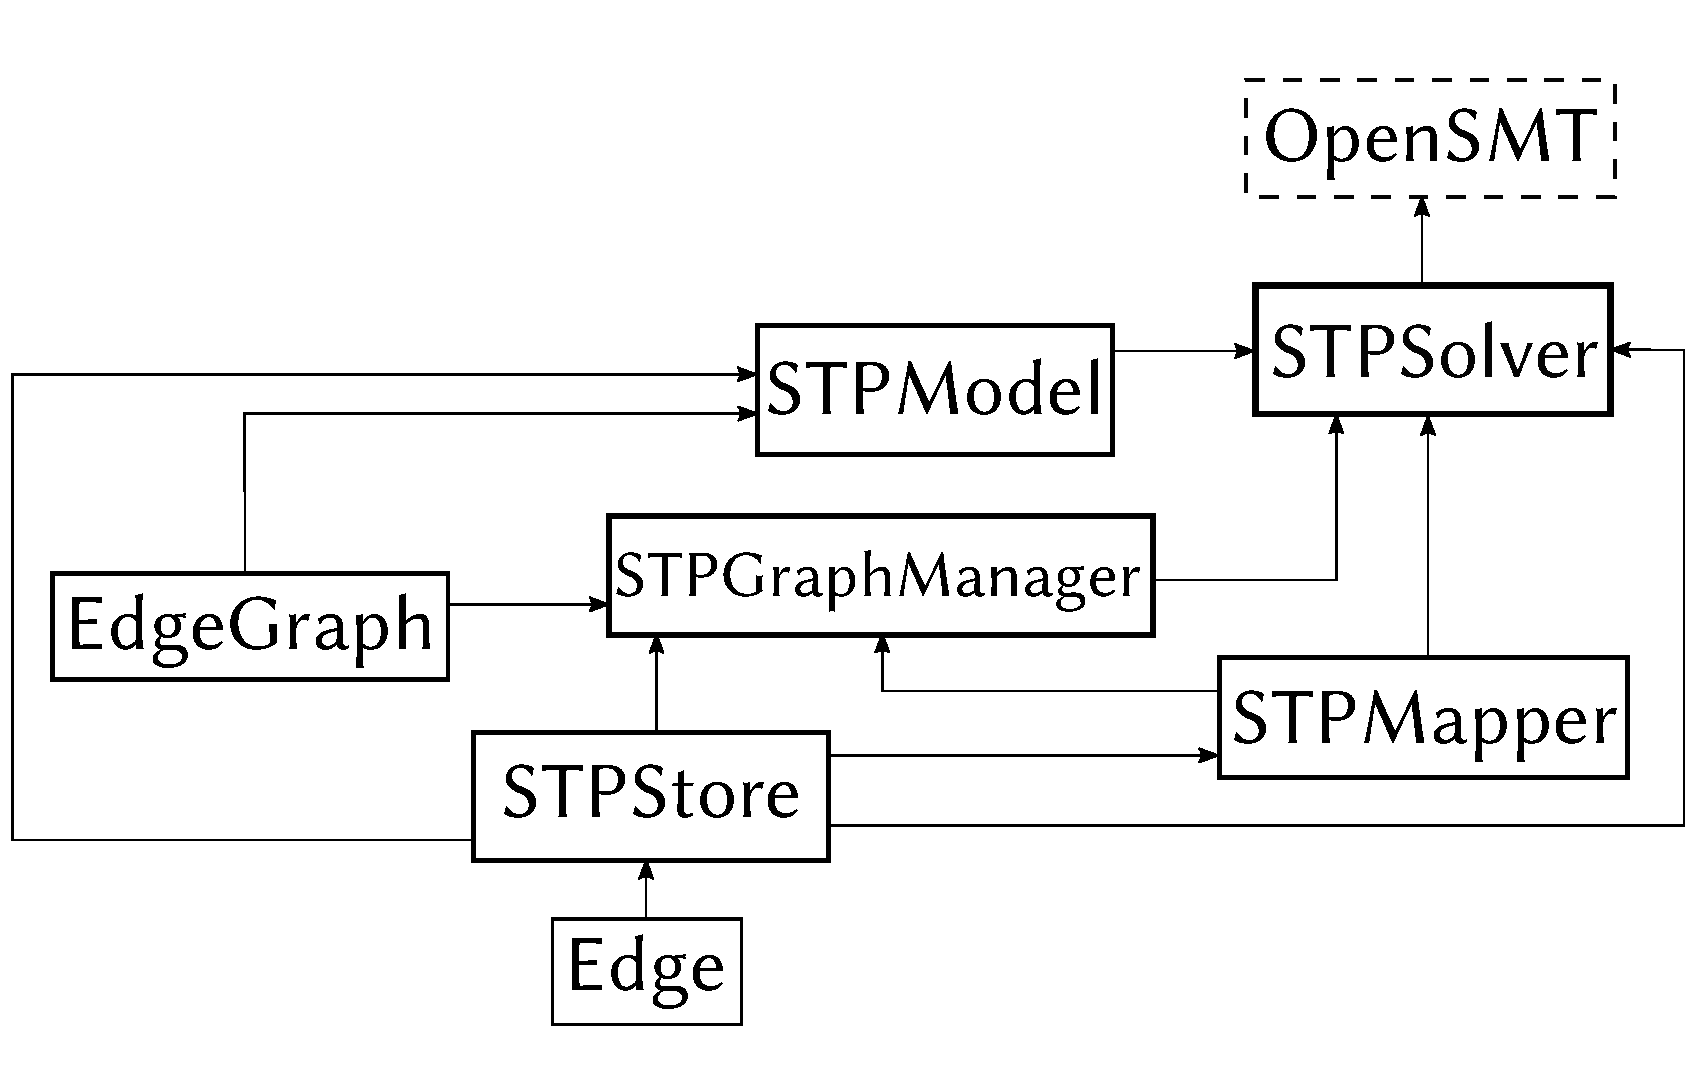
\includegraphics[width=0.8\textwidth]{class_deps}
	\caption{Závislosti mezi strukturami řešiče}
\end{figure}

Je vhodné zmínit, že za dobu vývoje OpenSMT v~něm vzniklo několik implementací základních datových struktur. Hojně užívaným příkladem je třída \icode{vec}, reprezentující běžný vektor. Vyjma malých rozdílů API a~údajné vyšší efektivity na primitivních typech se tyto třídy výrazně neliší od implementací ze standardní knihovny. Konkrétně třída \icode{vec} je navíc omezena skutečností, že jejími prvky nemohou být typy obsahující odkazy (vyjímkou z~tohoto pravidla je zvlášť implementovaný \icode{vec$\langle$vec$\langle$T$\rangle\rangle$}). Za účelem konzistence se zbytkem frameworku jsme se přesto rozhodli využívat tyto lokální struktury všude, kde je to možné. 


\section{Přidávání literálů}\label{add}

\section{Hledání důsledků}\label{dusl}

\section{Rozhodování o~splnitelnosti}

\section{Hledání konfliktů a~backtracking}

\section{Nalezení splňujícího ohodnocení}
